\documentclass[]{standalone}

%\usepackage{mathptmx}
%\renewcommand{\familydefault}{\rmdefault}
%\usepackage[T1]{fontenc}
%\usepackage[latin9]{inputenc}
\usepackage{siunitx}
\usepackage{array}
\usepackage{amsmath}
\usepackage{ifthen}
\usepackage{pgfplots}
\pgfplotsset{compat=1.14}
\usepackage{titling, graphicx}
\usepackage{tikz}
\usepackage{upgreek}
\usepackage{amsmath,amsthm}
\usepackage{strtikz}
\usepackage{circledsteps}
\usetikzlibrary{shapes,arrows.meta,intersections,graphs,graphs.standard}
\usetikzlibrary{bending, math,fit}
\usetikzlibrary{calc,intersections,through,backgrounds}
\usetikzlibrary{decorations.markings,decorations.pathmorphing, decorations.pathreplacing}
\usetikzlibrary{patterns}



\begin{document}



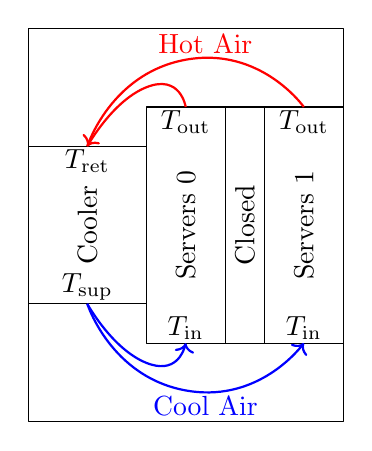
\begin{tikzpicture}[line join=round]

\draw (0,0) rectangle (4,5);

\draw (0,1.5) -- +(1.5,0);
\draw (0,3.5) -- +(1.5,0);

\draw (1.5,1.0) rectangle +(2.5,3);

\draw (2.5,1.0) -- +(0,3);
\draw (3.0,1.0) -- +(0,3);

\node (servers0) at (2.0, 2.5) [align=center, rotate=90] {Servers 0};
\node (servers0) at (2.75, 2.5) [align=center, rotate=90] {Closed};
\node (servers1) at (3.5, 2.5) [align=center, rotate=90] {Servers 1};

\node (cooler) at (0.75, 2.5) [align=center, rotate=90] {Cooler};

\draw[thick, blue, ->] plot [smooth, tension=1.25] coordinates {(0.75, 1.5) (1.5, 0.75) (2.0, 1.0)};
\draw[thick, blue, ->] plot [smooth, tension=1.25] coordinates {(0.75, 1.5) (2.0,0.4) (3.5, 1.0)};
\node (tsup) at (2.25, 0.20) [blue, align=center, inner sep=0] {Cool Air};
\node (t_sup) at (0.75, 1.5) [align=center, above, inner sep=1pt] {$T_\text{sup}$};
\node (t_in1) at (2, 1.0) [align=center, above, inner sep=1pt] {$T_\text{in}$};
\node (t_in1) at (3.5, 1.0) [align=center, above, inner sep=1pt] {$T_\text{in}$};


\begin{scope}[yshift=5cm, yscale=-1]
\draw[thick, red, <-] plot [smooth, tension=1.25] coordinates {(0.75, 1.5) (1.5, 0.75) (2.0, 1.0)};
\draw[thick, red, -] plot [smooth, tension=1.25] coordinates {(0.75, 1.5) (2.0,0.4) (3.5, 1.0)};
\node (tsup) at (2.25, 0.20) [red, align=center, inner sep=0] {Hot Air};
\node (t_sup) at (0.75, 1.5) [align=center, below, inner sep=1pt] {$T_\text{ret}$};
\node (t_in1) at (2, 1.0) [align=center, below, inner sep=1pt] {$T_\text{out}$};
\node (t_in1) at (3.5, 1.0) [align=center, below, inner sep=1pt] {$T_\text{out}$};
\end{scope}





\end{tikzpicture}




\end{document}
